\documentclass[12pt]{Qual}
\usepackage{preamble}

\name{Kayla Orlinsky}
\course{Complex Analysis Exam}
\term{Spring 2013}
\hwnum{Spring 2013}

\begin{document}

\begin{problem} $\,$
Evaluate $$\int_0^\infty\frac{x^{1/3}}{1+x^4}dx$$ being careful to justify your answer.
\end{problem}


\begin{solution}$\,$
We will use the contour around the top right quadrant avoiding the origin with the principal branch for $\frac{x^{1/3}}{1+x^4}$ being $(-\infty,0].$

\begin{center}
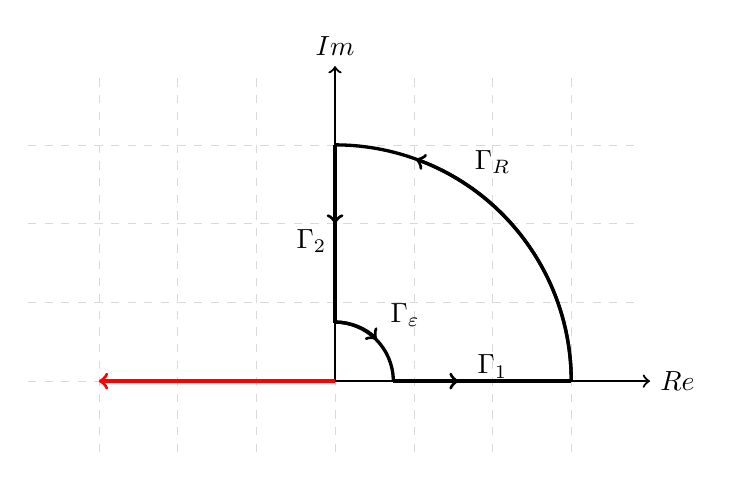
\begin{tikzpicture}
\draw[help lines, color=gray!30, dashed] (-3.9,-0.9) grid (3.9,3.9);
\draw[->,very thick] (3,0) arc (0:70:3cm);
\draw[very thick] (3,0) arc (0:90:3cm) node[above,yshift=-0.5cm,xshift=2cm]{$\Gamma_R$};
\draw[->,very thick] (0,0.75) arc (90:45:0.75cm);
\draw[very thick] (0.74,0) arc (0:90:0.75cm) node[above,yshift=-0.2cm,xshift=0.9cm]{$\Gamma_\varepsilon$};
\draw[->,very thick] (0.74,0) -- (1.57,0);
\draw[very thick] (0.75,0) -- (3,0) node[above,yshift=-0.1cm,xshift=-1cm]{$\Gamma_1$};
\draw[->,very thick] (0,3) -- (0,2);
\draw[very thick] (0,3) -- (0,0.74) node[above,yshift=0.75cm,xshift=-0.3cm]{$\Gamma_2$};
\draw[->, thick] (0,0)--(4,0) node[right]{$Re$};
\draw[->, thick] (0,0)--(0,4) node[above]{$Im$};
\draw[->,very thick,red] (0,0) -- (-3,0);
\end{tikzpicture}
\end{center}

Let \begin{align*}
    I_1&=\int_{\Gamma_1}\frac{z^{1/3}}{1+z^4}dz\\
    I_2&=\int_{\Gamma_2}\frac{z^{1/3}}{1+z^4}dz\\
    I_\varepsilon&=\int_{\Gamma_\varepsilon}\frac{z^{1/3}}{1+z^4}dz\\
    I_R&=\int_{\Gamma_R}\frac{z^{1/3}}{1+z^4}dz
\end{align*}

Now, \begin{align*}
    I_2&=\int_R^\varepsilon\frac{(ix)^{1/3}i}{1+x^4}dx\\
    &=\int_{R}^\varepsilon\frac{ie^{\frac{\pi i}{6}}x^{1/3}}{1+x^4}dx\\
    &=-ie^{\frac{\pi i}{6}}\int_\varepsilon^R\frac{x^{1/3}}{1+x^4}dx\\
    &=-ie^{\frac{\pi i}{6}}I_1
\end{align*}

Now, \begin{align*}
    |I_\varepsilon|&=\left|\int_{\Gamma_\varepsilon}\frac{z^{1/3}}{1+z^4}dz\right|\\
    &\le\int_{|z|=\varepsilon}\frac{\varepsilon^{1/3}}{|1+z^4|}|dz|\\
    &\le\int_{|z|=\varepsilon}\frac{\varepsilon^{1/3}}{1-\varepsilon^4}|dz|\\
    &=-\pi\varepsilon\frac{\varepsilon^{1/3}}{1-\varepsilon^4}\to0\qquad\varepsilon\to0.
\end{align*}

and similarly, \begin{align*}
    |I_R|&\le-\pi R\frac{R^{1/3}}{1-R^4}\\
    &=-\pi\frac{R^{4/3}}{1-R^4}\to0\qquad R\to\infty
\end{align*}

Finally, we note that there is one residue in the first quadrant since $$1+x^4=(i-x^2)(i+x^2)=(\sqrt{i}-x)(\sqrt{i}+x)(i\sqrt{i}+x)(i\sqrt{i}-x)\qquad\sqrt{i}=e^{i\pi/4}=\frac{\sqrt{2}}{2}+i\frac{\sqrt{2}}{2}$$ Alternatively, the zeros are $e^{ki\pi/4}$ for $k=1,3,5,7$ for which only the first is in the first quadrant.

Therefore, by the Residue Theorem, we get \begin{align*}
    2\pi i\res_{z=e^{i\pi/4}}\frac{z^{1/3}}{1+z^4}&=2\pi i\lim_{z\to e^{i\pi/4}}\frac{z^{1/3}(z-e^{i\pi/4})}{1+z^4}\\
    &=2\pi i\lim_{z\to e^{i\pi/4}}\frac{z^{4/3}-e^{i\pi/4}z^{1/3}}{1+z^4}\\
    &=2\pi i\lim_{z\to e^{i\pi/4}}\frac{\frac{4}{3}z^{1/3}-\frac{1}{3}e^{i\pi/4}z^{-2/3}}{4z^3}\qquad\text{L'Hopital's Rule}\\
    &=2\pi i\frac{\frac{4}{3}e^{i\pi/12}-\frac{1}{3}e^{i\pi/4}e^{-2i\pi/12}}{4e^{3i\pi/4}}\\
    &=2\pi i\frac{\frac{4}{3}e^{i\pi/12}-\frac{1}{3}e^{i\pi/12}}{4e^{3i\pi/4}}\\
    &=2\pi i\frac{e^{i\pi/12}}{4e^{3i\pi/4}}\\
    &=i\frac{\pi}{2}e^{-8i\pi /12}\\
    &=i\frac{\pi}{2}e^{-2i\pi /3}\\
    &=i\frac{\pi}{2}e^{4i\pi /3}\\
    &=\lim_{R\to\infty}\lim_{\varepsilon\to0}(I_1+I_2+I_\varepsilon+I_R)\\
    &=(1-ie^{\frac{\pi i}{6}})\int_0^\infty\frac{x^{1/3}}{1+x^4}dx\\
    \implies \int_0^\infty\frac{x^{1/3}}{1+x^4}dx&=\frac{i\frac{\pi}{2}e^{4i\pi /3}}{1-e^{4\pi i/6}}\\
    &=\frac{i\pi e^{4i\pi /3}}{2(1-e^{2\pi i/3})}\\
    &=\frac{i\pi}{2(e^{-4i\pi/3}-e^{-2i\pi/3})}\\
    &=\frac{\pi}{4}\frac{i2}{e^{2i\pi/3}-e^{-2i\pi/3}}\\
    &=\frac{\pi/4}{\sin(2\pi/3)}\\
    &=\frac{\pi/4}{\sqrt{3}/2}\\
    &=\frac{\pi}{2\sqrt{3}}
\end{align*}

\end{solution}
\newpage



\begin{problem} $\,$
Assume that $f$ is an entire function such that $$|f(z)|\ge\frac{1}{1+|z|}\qquad\text{ for all }z\in\mathbb{C}.$$ Prove that $f$ is a constant function.
\end{problem}

\begin{solution}$\,$
First, we note that $f(z)\not=0$ for all $|z|<\infty$ since $\frac{1}{1+|z|}>0$.

Thus, because $f$ is entire and non-zero, $g=\frac{1}{f}$ is entire and non-zero.

Thus, $$|g(z)|\le 1+|z|.$$ Therefore, by Cauchy Estimate, on $\{|z|\le R\}$, $$|g(z)|\le 1+|z|\le 1+R$$ and so $$|g^{(2)}(z)|\le \frac{2!(1+R)}{R^2}\to0\qquad R\to\infty.$$

Thus, $g(z)=az+b$, however, then $g(z)$ has a zero at $\frac{-b}{a}$ which is a contradiction unless $a=0.$

Namely, $g$ is constant and so $f$ is constant.
\end{solution}
\newpage




\begin{problem} $\,$
Let $f_n$, $n\ge1$, be a sequence of holomorphic functions on an open connected set $D$ such that $|f_n(z)|\le 1$ for all $z\in D$, $n\ge1$. Let $A\subset D$ be the set of all $z\in D$ for which the limit $\lim_nf_n(z)$ exists.

Show that if $A$ has an accumulation point in $D$, then there exists a holomoprhic function $f$ on $D$ such that $f_n\to f$ uniformly on every compact subset of $D$ as $n\to\infty.$
\end{problem}


\begin{solution}$\,$
Assume $A$ has an accumulation point in $z_0\in D.$

By Montel's theorem, since the $f_n$ are all uniformly bounded on $D$, $\{f_n\}$ form a normal family on $D$.

Thus, on every compact subset of $D$, there exists a holomorphic function $f$ such that there is a subsequence $\{f_{n_k}\}$ which converges uniformly to $f.$

We would like to show that the entire sequence $f_n\to f$ on each compact subset.

Let $f_{n_k}\to f$ on a compact subset $K\subset D$ containing $z_0$ which is the accumulation point of $A$ in $D$. Let $g_n=f_n-f$.

Then $g_{n-k}\to0$ uniformly on $K.$ Therefore, $g_n\to 0$ on $K\cap A$ since the limit exists and a subsequence converges to $0$.

Now, since $A\cap K$ contains an accumulation point, there is a sequence $\{z_l\}\subset A\cap K$ such that $z_l\to z_0$ and $\lim_{n\to\infty}g_n(z_l)=0$ for all $l$.

Now, since $\{f_n\}$ is uniformly bounded and holomorphic, by Arzela-Ascoli it is equicontinuous and so $\{g_n\}$ is equicontinuous. Let $\varepsilon>0$ be given and $\delta>0$ be such that $|g_n(z)-g_n(w)|<\varepsilon$ whenever $|z-w|<\delta.$

Therefore, if $\{B_{\delta/3}(z_l)\}$ is an open covering of some compact subset of $K$, then there exists a finite subcovering $B_{\delta/3}(z_{l_j})$. Now, since $g_n\to0$ pointwise on $K$, for each $z_{l_j}$ take $N_j$ such that $|g_n(z_{l_j})|<\varepsilon$ for all $n\ge N_j$.

Let $N$ be the maximimum of the $N_j$. Then for $z$ in this finite subcovering, there is a $z_{l_j}$ such that $|z-z_{l_j}|<\delta$ and so $$|g_n(z)|\le|g_n(z)-g_n(z_{l_j})|+|g_n(z_{l_j})|<\varepsilon+\varepsilon$$ for all $n\ge N$.

Thus, $g_n\to0$ uniformly on some compact subset of $K.$ However, this can clearly be extended to all of $K$ and therefore to any compact subset of $D$ using similar open coverings.

and so $g_n(z)\to0$ uniformly on compact subsets of $D$. Thus, $f_n\to f$ uniofmrly on compact subsets of $D.$
\end{solution}
\newpage





\begin{problem} $\,$
Let $f(z)$ be meromorphic on $\mathbb{C}$, holomoprhic for $Re z>0$ and such that $f(z+1)=zf(z)$ in its domain with $f(1)=1$. Show that $f$ has the first order poles at $0,-1,-2,...,$ and find the residues of $f$ at these points.
\end{problem}


\begin{solution}$\,$
$f(1)=f(0+1)=1$ implies that $$\lim_{z\to0}zf(z)=1.$$ Namely, that $f$ has a first order pole (else the limit would be $0$ or infinity) at $0$ of residue $1.$

Now, $$\lim_{z\to-1}(z+1)f(z)=\lim_{z\to-1}(z+1)\frac{f(z+1)}{z}=\lim_{w\to0}\frac{wf(w)}{w-1}=\frac{1}{-1}=-1$$ and so $f$ has a first order pole at $-1$ of residue $-1.$

Similarly, since $$f(z)=\frac{f(z+1)}{z}=\frac{f(z+2)}{z(z+1)}=\frac{f(z+n)}{z(z+1)\cdots(z+n-1)}$$ we get that $$\lim_{z\to-n}(z+n)f(z)=\lim_{z\to-n}\frac{(z+n)f(z+n)}{z(z+1)\cdots(z+n-1)}=\lim_{w\to0}\frac{wf(w)}{(w-n)(w-n+1)\cdots(w-1)}=\frac{1}{(-n)(-n+1)\cdots(-1)}.$$

Since all these poles are first order (as evidenced by the limit), these limits correspond exactly to the residues and so $f$ has first order poles at $-n$ for all $n\in\mathbb{N}$ with residue $\frac{1}{(-n)(-n+1)\cdots(-1)}$ and a first order pole at $0$ with residue $1.$
\end{solution}


\end{document}
